\documentclass[main.tex]{subfiles}
 
\begin{document}
The goal of the model described in this thesis can be summarised as follows:


\textbf{Given:}
\begin{itemize}
    \item A real-world \emph{grid structure}
    \item Hourly \emph{load series}
    \item Hourly \emph{generation series}
\end{itemize}

\textbf{Predict:}
\begin{itemize}
    \item \emph{`Top 10'} of lines most likely to fail
    \item For each risky line: the most likely \emph{cascading line failures}
\end{itemize}

The model, in particular the use of large deviation statistics to study cascading line failures, was proposed by \citet{Nesti2018emergentfailures}.\nocite{Nesti2018supplemental} Following their approach, the model is applied numerically to the SciGRID dataset \citep{SciGRIDv0.2}. This dataset is an approximation of the transmission network in Germany, including grid structure, generation capacity, hourly load series and hourly renewable generation series.

As discussed in Section \ref{linefailurecauses}, transmission lines can fail for a number of reasons, and this model only studies one specific type of failure: \emph{short-term changes in renewable generation}.
\todo{how common are these types of failures?}






Line overloads are, however, the most imminent type of failure in a network, in the sense that grid operators need to continually monitor the \define{configuration} (distribution among the nodes of power generation) to ensure that no line will overload.
This strongly constrains the capability of the transmission network. At any point in time, there could be many configurations that are environmentally (or \emph{economically}) better than the current configuration, but they might lead to a line overload.%
\footnote{It is for this reason that the Optimal Power Flow problem is computationally difficult solve: it often takes many iterations until a generation distribution is found that does not cause any transmission line to be overloaded.}
Turning off functioning wind turbines is known as \emph{wind curtailment}\index{curtailment!wind}, and switching off solar panels is called \emph{solar curtailment}\index{curtailment!solar}.%
\footnote{Wind turbines can indeed be turned off, by twisting the rotor blades towards $0\si{\degree}$ pitch and applying the \emph{brakes}. In larger turbines, common types are drum brakes (similar to a back-pedalling brake for bikes) and disk brakes. Brakes are especially important during maintenance.
Solar panels are switched off using a simple mechanical or electronic switch (a relay). (\cite{Denholm2015})}

In China, as of 2019 the world's largest producer of renewable energy \emph{by a factor of two}, \tocite{ref, wiki} wind curtailment amounted to 16\% between 2010 and 2016. (\cite{Qi2018})



\section{Constructing a complete dataset}
\subsection{PyPSA \& SciGRID}
Asdf
\towrite{context, }
\tocite{context: PSAT for matlab \cite{Milano2005}, references 110 and 111 of PSAT manual \cite{Milano2013PSATManual}}
\towrite{some example graphs}
\tocite{PyPSA: \cite{PyPSA}}
\tocite{Maybe: PyPSA-EUR: \cite{PyPSAEUR}}
\section{LPF}
\subsection{Comparison with PyPSA results}
\begin{figure}
    \centering
    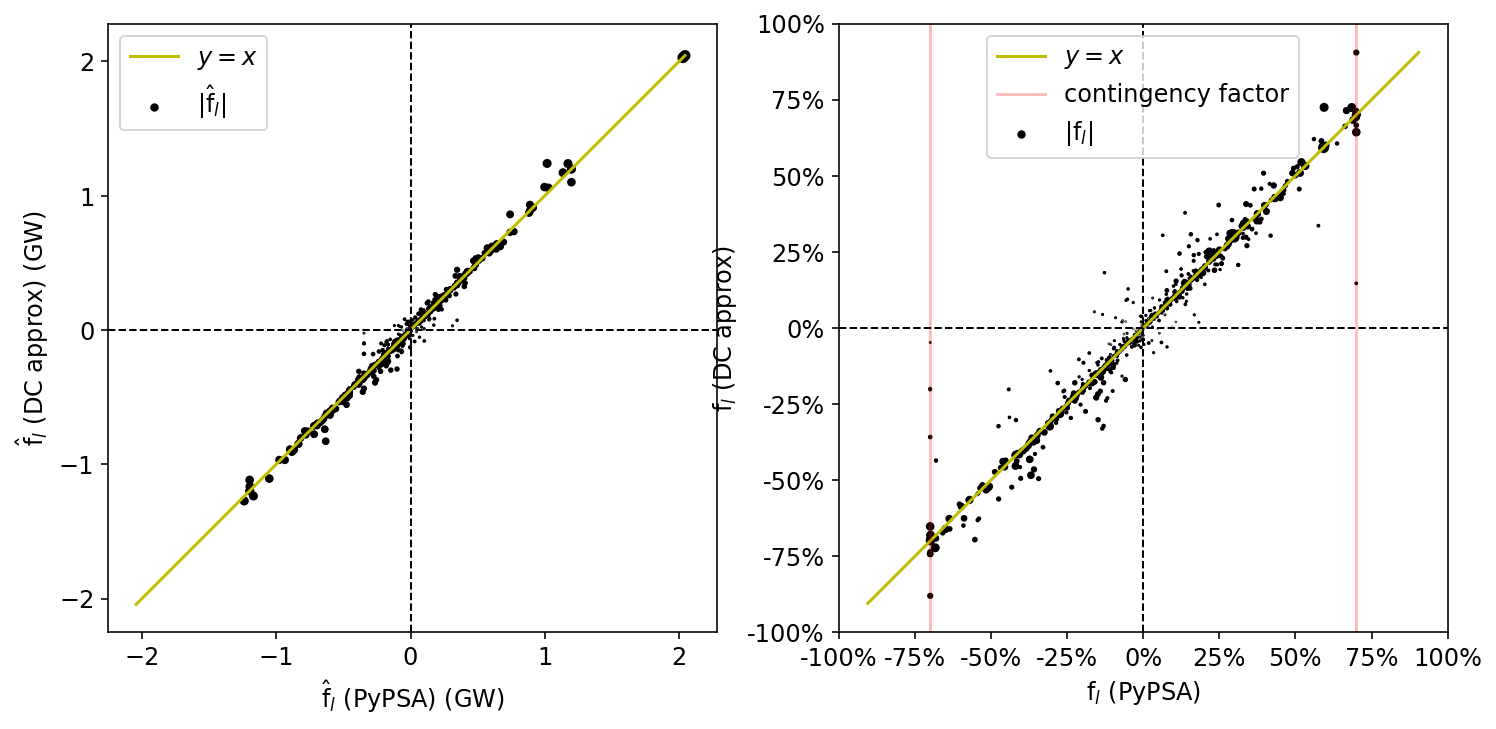
\includegraphics[width=\textwidth]{img/lineflowcorr.png}
    \caption{PLACEHOLDER: Line flow (left) and saturation (right) computed using LPF and (non-linear) PF.}
    \label{fig:generationtech}
\end{figure}
\section{Stochastic power injection}
\subsection{Explorative data analysis}
\subsection{ARMA model}

\subsubsection{Computing ARMA fits}\label{arimamod}
Following \cite{Nesti2018emergentfailures}, the ARMA models were fitted to the first month of solar and wind generation series using the \texttt{arima} method in \texttt{R}. This produced the desired result for all wind series.

Unfortunately, the \texttt{arima} method failed to fit an ARMA model for 104 of the 489 buses, reflecting the hypothesis that these series are poorly modelled by an ARMA series. To recreate the results of \cite{Nesti2018emergentfailures}, it is crucial that a model can be fitted for \emph{every} bus. Therefore, a modified method is required.

By the default, the \texttt{arima} method operates in two steps. First, a so-called Conditional-Sum-of-Squares (CSS) method is used as initial guess for the ARMA coefficients. Then, the coefficient \emph{likelihood} function is maximised with the Nelder-Mead optimisation method, using the CSS result as initial value. 

In our case, the CSS method often finds initial values that are \emph{non-stationary}.\todo{define?} A possible reason is that solar generation is exactly zero during nighttime, which lasts for up to 16 consecutive hours.\footnote{In reality, solar generation is never \emph{exactly} zero, even after sunset, because solar panels also receive ambient light. This is not included in the (artificial) dataset.
%Ambient light includes sunlight scattered by the atmosphere (\eg 3 hours of twilight in January), artificial light 
%TODO
}
To resolve this issue, we use an optimisation method that works well without specifying an initial value: it should find the \emph{global} maximum independently. The Simulated Annealing (SANN) algorithm included in \texttt{R} is such a method, and was chosen for this analysis. 

With SANN as optimisation method, \texttt{arima} was able to fit solar models for 484 out of 489 buses. For the remaining 5 buses, a second technique is applied: to accommodate for the long periods of zero generation, a small amount of uniform noise is superimposed on the generation series. Initially, the noise magnitude is set to 1\% of the solar capacity of the bus. This percentage is increased iteratively, until the modified method is able to fit a solar model. In fact, 1\% noise proved sufficient for the remaining 5 buses in January, and no more than 2\% noise was needed for any bus in the remaining months. 

The modified method described in this section was used to fit solar and wind models to each bus of the network, for each month of 2011. Table \ref{tab:arimafitstats} lists the number of buses that can be analysed using the default and modified methods, showing the poor performance of the default for solar series, especially during the months of summer.
\tocite{Belisle 1992, zie \texttt{optim} docs}

\citet{Nesti2018emergentfailures} do not mention such problems (nor techniques to solve them). Because the same dataset, processing, programming language and method was used in this analysis, it is likely that they have also encountered and solved these problems, possibly in the same manner.
\towrite{discuss other possible techniques: warm start, intercept}

\subsubsection{Runtime}
The default implementation has an estimated (single-core) runtime of 101 hours (4.2 days) when all 12 months are analysed, although only 78\% of fits are successful using this method.

The modified version is able to fit all generation series successfully. The use of this more computationally expensive method increases the runtime to an estimated 224 hours (9.4 days). Because of the long runtime, fits were computed in parallel on a 40-core machine\footnote{Specifications: two \textit{Intel Xeon E5 2630L v4} 10-core processors @2GHz with hyperthreading; 64GB RAM. CPU time was used as estimate for single-core runtime.}, provided by the IT department of the Radboud University.\footnote{Thank you!} This reduced the total runtime down to 7 hours. The results are publicly available at the GitHub repository.

\subsection{Stochastic line flows}

\section{Line failures}
\section{Cascading line failures}
\end{document}